\section{Methodik}

\subsection{Beschreibung der Datenquelle und -beschaffung}

\subsection{Auswahl der Technologien}
Die Auswahl der geeigneten Technologien für die Entwicklung des innovativen 
Studiengangsfinders wurde sorgfältig überlegt, um eine effiziente und
interaktive Lösung zu gewährleisten. Besonders wichtig ist die Nutzbarkeit auf
Smartphones und Desktop-Geräten, wodurch sich außerdem neue Herausforderungen
hinsichtlich der Bedienung ergeben. Im Folgenden werden die Hauptkomponenten des
Technologiestacks und ihre jeweiligen Funktionen erläutert.

\subsubsection{Interaktive Grafik (Frontend)}
Für die Darstellung der interaktiven Grafik wurde Pixi.js gewählt. Pixi.js ist
ein leistungsstarkes WebGL-Rendering-Framework, das eine schnelle und
reibungslose Darstellung von Grafiken ermöglicht. \parencite{pixijs} Die
Entscheidung für Pixi.js basiert auf seiner Effizienz bei der Verarbeitung
komplexer 2D-Grafiken und seiner Fähigkeit, eine ansprechende Benutzererfahrung
zu bieten.

Neben Pixi.js wurden verschiedene weitere Bibliotheken betrachtet:
\begin{itemize}
    \item three.js: WebGL 3D-Framework
    \item D3.js: 2D-Datenvisualisierungsbibliothek
    \item Chart.js: HTML5-Bibliothek für Diagramme
    \item Paper.js: HTML5-Bibliothek für Animationen und interaktive Grafiken
    \item Fabric.js: 2D-Canvas Bibliothek
\end{itemize}

% TODO: Quellen für die "Forenthreads" gegen die Frameworks etc verlinken

Der Studiengangsfinder erfordert eine 2D-Grafikdarstellung, weshalb
\textit{three.js}, das auf 3D-Visualisierungen spezialisiert ist, nicht als
geeignete Grundlage gewählt wurde. \parencite{threejs}

Die Entscheidung gegen die Verwendung von \textit{D3.js} wurde aufgrund
von Bedenken bezüglich der Dokumentation und der Wahrnehmung in der 
Entwicklergemeinschaft getroffen. Die unvollständige Dokumentation und
bestehende Forenthreads, die die Relevanz von D3.js in Frage stellen, könnten zu
potenziellen Schwierigkeiten bei der Entwicklung und zukünftigen Wartungen
führen. \parencite{d3js}

% d3js-trend, d3js-trend-2

Aufgrund der festgestellten Einschränkungen in der Flexibilität von
\textit{Chart.js} wurde gegen die Verwendung der Bibliothek entschieden. Obwohl
Chart.js die Erstellung einer Vielzahl von Diagrammen ermöglicht, hat sich
gezeigt, dass die Anpassbarkeit eingeschränkt ist. \parencite{chartjs}

Basierend auf der wahrgenommenen Inaktivität des Projekts und den festgestellten 
Einschränkungen in Bezug auf Event-Handler wurde entschieden, \textit{Paper.js}
nicht zu verwenden. \parencite{paperjs} Die begrenzten Event-Handler schränken
die Interaktionsmöglichkeiten ein, was im Kontext des Studiengangsfinders, der
eine umfassende Benutzerinteraktion für Smartphone und Desktop-Gerät erfordert,
als unzureichend erachtet wurde. \parencite{paperjs-events}

Obwohl \textit{Fabric.js} als vielversprechende Alternative erschien, wurde
Pixi.js aufgrund mehrerer Faktoren bevorzugt \parencite{fabricjs}. Der
professionellere Website-Auftritt von Pixi.js trug dazu bei, das Vertrauen in
die Zuverlässigkeit und Wartbarkeit des Frameworks zu stärken. Ein weiterer
bedeutender Punkt ist die Anzahl der GitHub-Sterne in Relation zu der Anzahl an
\textit{offenen Issues}, die Pixi.js aufweist. Eine höhere Anzahl an
GitHub-Sternen mit gleichzeitig weniger offenen Issues, deutet oft auf eine
größere und aktivere Entwicklergemeinschaft hin, was wiederum auf
kontinuierliche Weiterentwicklung und Wartung schließen lässt.
\parencite{paperjs-pixijs-comparison}


\subsection{Beschreibung der Algorithmen}
Der Studiengangsfinder soll Studieninteressierten einen schnellen Überblick über
alle in Frage kommenden Studiengänge ermöglichen.  Dabei soll dem Nutzer eine
interaktive Grafik präsentiert werden, mit der er anhand von Studieninhalten
(z.B. \glqq Gesundheit und Soziales\grqq{}) sofort alle relevanten Studiengänge
findet. Dazu ist es notwendig, die Studiengänge nach ihren Inhalten zu
gruppieren (Clustering) und schließlich visuell ästhetisch aufzubereiten.

Bei der Festlegung des Clustering-Algorithmus für den Studiengangfinder wurden
verschiedene Optionen in Betracht gezogen, darunter K-Means Clustering,
Force-Directed Layouts und Multidimensionale Skalierung (MDS). Nach einer
gründlichen Abwägung der Vor- und Nachteile fiel die Wahl auf MDS. Die Gründe
für diese Entscheidung und eine Erläuterung der jeweiligen Algorithmen werden in
den folgenden Kapiteln gegeben.

\subsubsection{Force-Directed-Graphs}
Force-Directed Graph Drawing ist eine Methode zur Visualisierung von Graphen,
bei der die Positionen der Knoten und Kanten aufgrund von Kräften bestimmt
werden. Das Vorgehen hierbei ist vereinfacht inspiriert von Modellen der
Teilchenphysik und wird häufig mit dem Verhalten von Federn verglichen. Ziel des
Algorithmus ist es durch Kanten verbundene Knoten nah beinander zu platzieren
und somit eine ästhetisch ansprechende Visualisierung eines Graphen zu
berechnen. In \autoref{fig:force-directed-layouts} erkennt man ausgehend von
einer zufälligen Positionierung (Zustand 0), eine schrittweise Optimierung der
Darstellung. Wie stark oder schwach sich die Knoten jeweils
\glqq anziehen\grqq{} bzw. \glqq abstoßen\grqq{} wird durch die Gleichmäßigkeit
der Verteilung auf der sogenannten Zeichenfläche bestimmt.
\parencite{force-directed-layouts}

\begin{figure}[H]
    \centering
    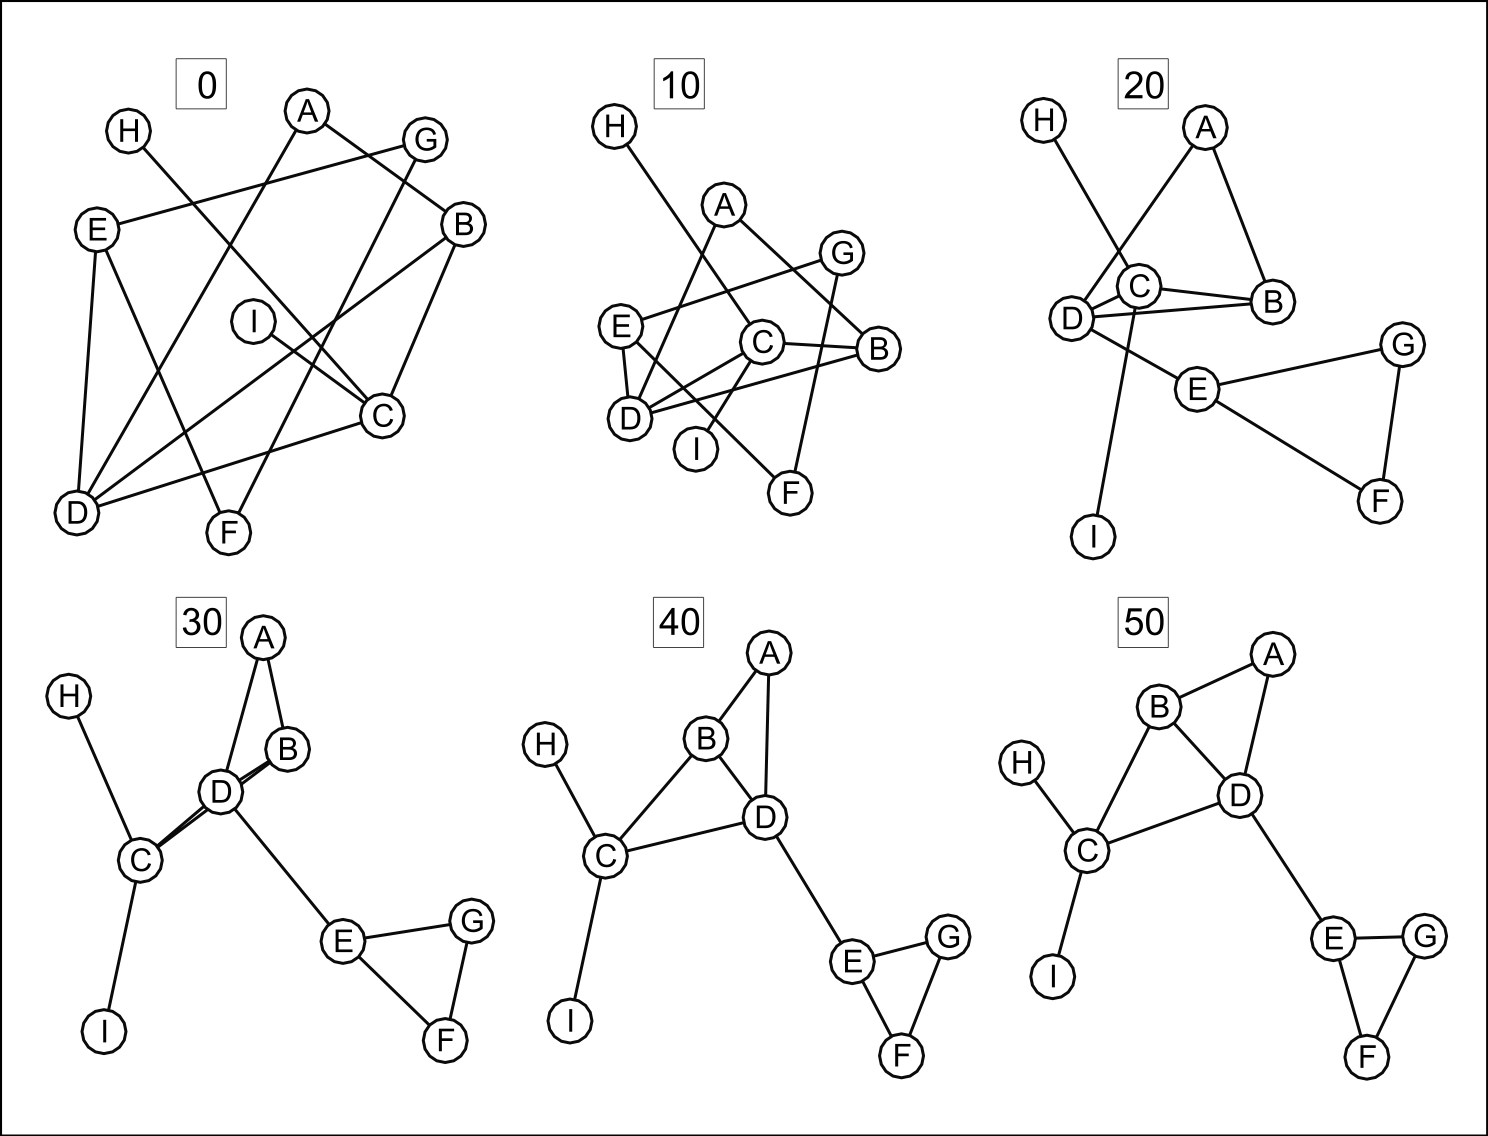
\includegraphics[width=\textwidth]{force-directed-layouts}
    \caption{Schrittweises Durchführen des Layout-Algorithmus von Fruchterman/Reingold}
    \bildquelle{Fruchterman, Thomas M. J./Reingold, Edward M.: Graph Drawing by Force-Directed Placement}
    \label{fig:force-directed-layouts}
\end{figure}

Force-Directed Layouts sind besonders effektiv für die übersichtliche
Darstellung von Netzwerken, in denen die Verbindungen zwischen den Elementen im
Vordergrund stehen. \parencite{force-directed-layouts} Im Gegensatz dazu
erfordert der Studiengangsfinder eine kontinuierliche Positionierung der
Studiengänge basierend auf inhaltlichen Ähnlichkeiten, was nicht unbedingt der
Stärke von Force-Directed Layouts entspricht. Force-Directed Graph Drawing
benötigt als Vorraussetzung bereits einen Graphen mit Knoten und Kanten, welche
im Fall des Studiengangsfinders die Ähnlichkeiten zwischen den einzelnen
Studiengängen entsprechen würde. Gerade die Berechnung der Ähnlichkeit zwischen
den einzelnen Studiengängen ist jedoch wesentlicher Bestandteil dieser Arbeit,
weshalb der Algorithmus nicht näher untersucht wurde.

\subsubsection{K-Means Clustering Algorithmus}
K-Means ist ein Clustering-Algorithmus, der Datenpunkte in k vordefinierte
Gruppen oder Cluster einteilt. Die Wahl von K stellt die Anzahl der Cluster dar,
und der Algorithmus versucht, die Datenpunkte so zu gruppieren, dass die Varianz
innerhalb der Cluster minimiert wird (siehe \autoref{fig:kmeans}).
\parencite{kmeans}

\begin{figure}[H]
    \centering
    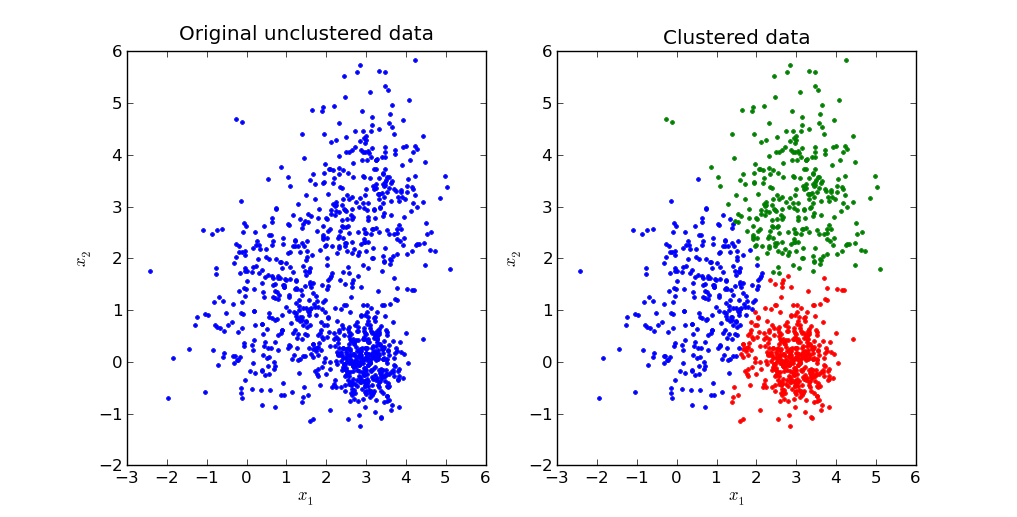
\includegraphics[width=\textwidth]{kmeans}
    \caption{K-Means Clustering Algorithmus}
    \bildquelle{https://mubaris.com/posts/kmeans-clustering/}
    \label{fig:kmeans}
\end{figure}

Die Entscheidung, den K-Means-Algorithmus nicht zu verwenden, basiert darauf,
dass dieser hauptsächlich darauf abzielt, Datenpunkte zu gruppieren und weniger
auf deren präzise Positionierung in einem zweidimensionalen Raum. Der
Algorithmus fordert außerdem eine vordefinierte Clusteranzahl k. Das stellt im
Falle des Studiengangsfinders jedoch keine Einschränkung dar, da jeder Cluster
eine Inhaltskategorie, wie zum Beispiel \glqq Informatik\grqq{} repräsentieren
würde. Trotzdem erweist sich der K-Means Clustering Algorithmus als unpassend,
da er sehr empfindlich gegenüber Ausreißern ist, da er versucht, Clusterzentren
zu finden, die die Gesamtvarianz minimieren. Wenn es Ausreißer in den
Studienschwerpunkten gibt, könnten sie das Ergebnis beeinflussen.
\parencite{kmeans-spikes}

Insgesamt erfüllt der MDS-Algorithmus die spezifischen Anforderungen des
Studiengangsfinders, indem er eine übersichtliche und interpretierbare
Visualisierung der Studiengänge basierend auf inhaltlichen Ähnlichkeiten
ermöglicht.

\subsubsection{Multidimensionale Skalierung (MDS)}
MDS ermöglicht die Reduktion n-dimensionaler Daten auf zwei oder drei
Dimensionen, wodurch eine anschauliche Darstellung in Form von Koordinatenpaaren
ermöglicht wird. Dieser Aspekt ist entscheidend, um Studiengänge in einem
zweidimensionalen Diagramm zu positionieren, wobei ähnliche Studiengänge
aufgrund ihrer inhaltlichen Ähnlichkeiten nahe beieinander liegen. Die Anwendung
des MDS-Algorithmus auf eine genormte Tabelle, in der die Studiengänge nach
ihren Anteilen an verschiedenen Inhaltskategorien gewichtet sind, ermöglicht
eine effektive Positionierung im Diagramm.
